\subsubsection*{AlphaGo Zero} AlphaGo Zero\cite{b35} was developed after the Chinese Summit. While AlphaGo learned the game by playing thousands of matches with amateur and professional players, AlphaGo Zero learned by playing against itself (starting from completely random play). This powerful technique successfully accumulated thousands of years of human knowledge by training for just a few days. It quickly surpassed all previous versions' performance and discovered new knowledge, developing unconventional strategies and intuitive new moves. 

\subsubsection*{AlphaZero} AlphaZero\cite{b36} was introduced in late 2017. It mastered the games of chess, shogi, and Go by learning from scratch (beating a world-champion computer program in each case). It replaces hand-crafted heuristics with a deep neural network and algorithms that are given only the basic rules. 
% E.g., in its chess games, players saw that it had developed a highly dynamic and unconventional style that differed from any previous chess-playing engine.  

\subsubsection*{MuZero} MuZero\cite{b13} is the latest version of the AlphaGo family. It takes these ideas of AlphaZero one step further. It is a new approach to model-based RL. It achieves state-of-the-art performances in Atari 2600 games as well in chess, shogi, and Go, without prior knowledge of the game dynamics. It uses AlphaZero's powerful search and policy iteration algorithms and incorporates the learned model into the training procedure. It extends to a broader set of environments, including single-agent domains and non-zero rewards at intermediate time steps. It allows planning winning strategies in unknown domains, a significant leap forward in the capabilities of RL algorithms, and an essential step towards building general-purpose learning systems.  

\begin{figure}[t]
    \centering
    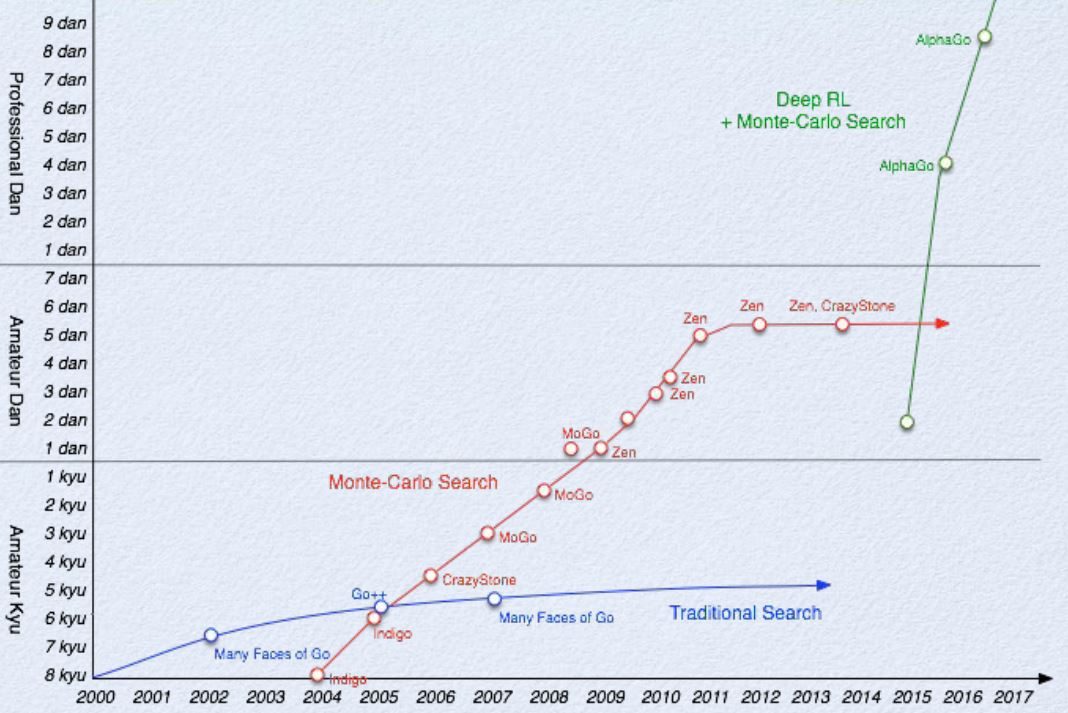
\includegraphics[width = 0.7\columnwidth]{Con_2.2}
    \caption{Progress in Computer Go\cite{b26}}
    \label{Prog_comp_go}
\end{figure}